\documentclass[10pt,a4paper,twocolumn]{article}
\usepackage[utf8]{inputenc}
\usepackage[T1]{fontenc}
\usepackage{times}
\usepackage[left=0.8cm,top=0.8cm,right=0.8cm,bottom=0.8cm]{geometry}
\usepackage{amsmath}
\usepackage{amssymb}
\usepackage{makeidx}
\usepackage{graphicx}
\usepackage{hyperref}
\usepackage{float}
\usepackage{indentfirst}
\usepackage[portuguese]{babel}

\pagestyle{empty}
\title{\textbf{Diodos aplicados à sensores digitais de imagem}}
\author{Leandro Assis dos Santos}

\linespread{0.835}
\setlength{\parskip}{0.028cm}

\begin{document}
\pagestyle{empty}
\maketitle

\section*{Introdução}
		Sensores digitais de imagem são sensores que transdutam a intensidade luminosa incidente sobre eles em sinais elétricos analizáveis por um sistema computacional. Esses sensores são usados em imagens eletrônicas aplicadas à diversos dispositivos como câmeras digitais, mouses ópticos, equipamentos de imagem médica, equipamentos de visão noturna e térmica, LIDARs (Light Detection and Ranging), dentre outros.
				
		Em resumo, a aplicação de diodos em câmeras digitais é possibilidade pois ao polarizar um diodo reversamente com uma fonte de tensão $V$ como na Figura 1, o campo elétrico interno da junção pn que constitui o diodo é reforçado. Por conta disso, a barreira de potencial se fortalece e mais íons (de ambos, aceitadores e doadores) ficam expostos. Devido ao campo induzido pelo terminal positivo da fonte $V$, os elétrons livres são atraídos para o extremo do cátodo do diodo, e por consequência as lacunas são direciondas para o anôdo do componente.
		
		\begin{figure}[!h]
			\centering
			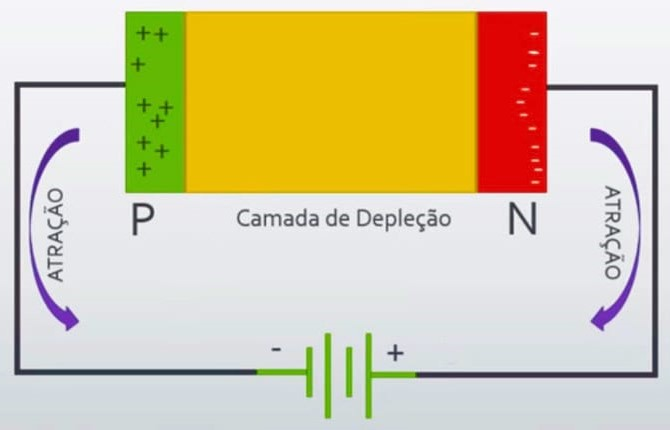
\includegraphics[scale=0.2]{imagens/diodo_polarizado_reversamente.jpg}
			\caption{Diodo polarizado reversamente.}
		\end{figure}
		Em razão da concentração de cargas nos extremos do diodo e do aumento da barreira de potencial, isto é, o aumento da voltagem entre as extremidades da região de depleção por conta dos íons expostos, a região de depleção se torna mais larga e podemos pensar nos extremos do diodo como as placas de um capacitor. A junção pn portanto, quando polarizada reversamente, possui capacitância dependente de $V$.
		
		Uma vez que se possui o fótodiodo funcionando como um capacitor sob uma tensão reversa, o dispositivo se carregará com um dado valor $V_{C}$ que depende do tempo ao qual o fótodiodo (agora agindo como capacitor) ficou alimentado pela tensão reversa $V$. Com o fótodiodo carregado permite-se a entrada de luz sobre o sensor, que resultará em uma indução de corrente na junção pn e, consequentemente, em uma diminuição na tensão $V_{C}$. A partir da observação individual da tensão $V_{C}$ em uma matriz de fótodiodos é possível fazer a transdução da luz incidente sobre o sensor em uma imagem.
		
\section*{Tipos de sensores de imagem}
		Os sensores de imagem podem ser separados em dois principais tipos, eles são os CCDs (\textit{Charge-Couple Device}) e os sensores CMOS, configuração de sensor baseada em APS (\textit{Active Pixel Sensor}), podendo ser classificados de acordo com o número de transistores por pixel, como por exemplo 3T-APS, 4T-APS e assim por diante. Ambos os dispositivos são feitos com tecnologia MOS (\textit{Metal Oxide Semiconductor}), com CCDs baseados em capacitores MOS e os sensores CMOS baseados em amplificadores MOSFET. A seguir entra-se em mais detalhes sobre cada tipo de sensor, suas características, histórias, vantagens e desvantagens.
		
	\subsection*{A história dos sensores de imagem}
		Os sensores CCDs são pioneiros no ramo de imagem digital e sua origem remonta às pesquisas com tecnologia MOS de Willard Boyle e George E. Smith. Durante a pesquisa descobriram que uma carga elétrica poderia ser armazenada em pequenos capacitores MOS, descoberta essa que se tornou a base para o sensor CCD, inventado em 1969.
		
		Os CCDs fabricados na época sofriam de distorções causadas pelo atraso do obturador das câmeras. Distorções que foram resolvidas apenas em 1980 quando surgiu um dispositivo que viria a ser o fator chave para os sensores CMOS modernos, o fótodiodo ``fixado'' (do inglês PPD - Pinned PhotoDiode) inventado por Nobukazu Teranishi, Hiromitsu Shiraki e Yasuo Ishihara. O diferencial desse componente em relação aos demais é o baixo \textit{lag}, baixo ruído, alta eficiência quântica (taxa de conversão de fótons em elétrons) e baixa corrente quando aplicado a pouca luminosidade (\textit{dark current}). A partir de 1987, os PPDs começaram a ser incorporados na maioria dos sensores CCDs, e desde então são usados em todos os sensores CCD e CMOS.
		
		A tecnologia base para os pixels de sensores CMOS foi inventada pela Olympus em meados dos anos 80. Essa tecnologia foi possibilitada pelos avanços na tecnologia de fabricação de semicondutores MOS, com MOSFETs atingindo escalas de mécrons e submícrons de tamanho. O primeiro sensor ``parente'' dos sensores CMOS foi fabricado por Tsutomu Nakamura e sua equipe em 1985 utilizando transistores NMOS. Posteriormente, os sensores CMOS, como conhecido, hoje foi desenvolvido por Eric Fossum e sua equipe nos laboratórios da NASA em 1993.
		
		\begin{figure}[H]
		\centering
		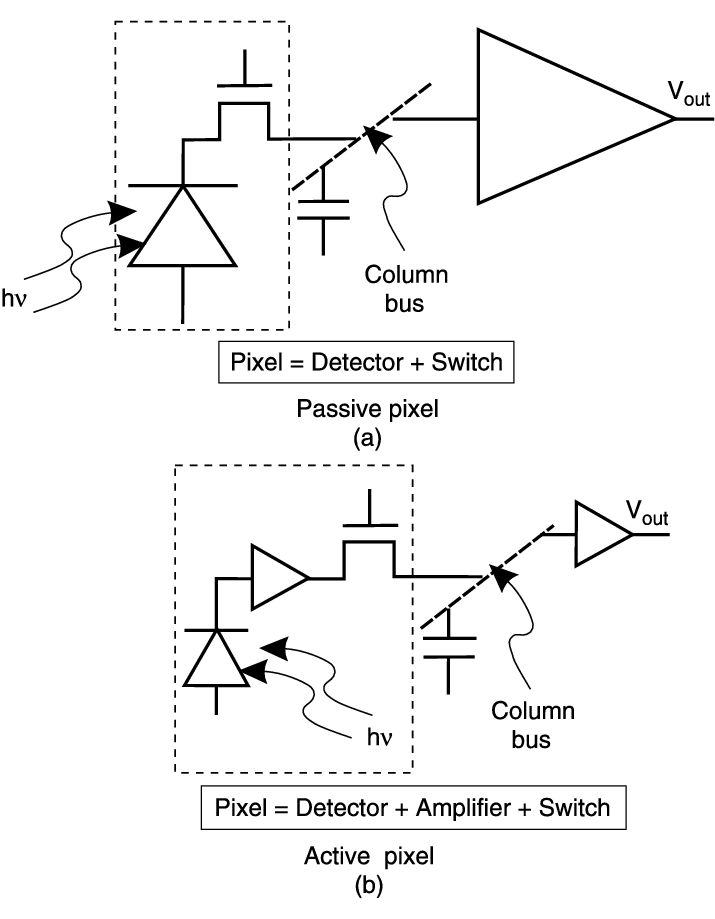
\includegraphics[scale=0.22]{imagens/passive_vs_active.png}
		\caption{Apresentação das configurações de PPS (a) e APS (b).}
		\end{figure}
		
	\subsubsection*{Sensores de Pixel Passivo - PPS} 
		Os precursores dos sensores APS foram os PPS (do inglês, passive-pixel sensor), um tipo de matriz de pixels formada por fótodiodos e uma chave MOSFET, que consiste em ``pixels passivos'' sem amplificação, ou seja, essa configuração de pixel transfere diretamente o sinal acumulado para fora do pixel. Nesses sensores, cada pixel possui uma junção pn e transistores de seleção. Essa configuração de pixels passivos foi proposta por G. Weckler em 1968 e antecedeu a criação dos CCDs. Os PPS sofrem de limitações como baixo tempo de leitura e dificuldade de escalabilidade. De forma geral, os sensores CCDs possuem matrizes de pixels passivos.
		
	\subsubsection*{Sensores de Pixel Ativos - APS}
		Esses sensores consistem de ``pixels ativos'', que consistem em um ou mais amplificadores MOSFET que convertem a carga fótogerada no fótodiodo em uma tensão de saída. Esse conceito de pixel foi proposto por Peter Noble em 1968, entretanto, como dito anteriormente, esta topologia de pixels só foi fabricada a partir de 1985 devido as evoluções nos processos de fabricação dos transistores MOS.  Os sensores CMOS utilizam dessa configuração de pixels para seu funcionamento, tendo como principal diferença o uso de transistores CMOS ao invés de transistores PMOS ou NMOS.
	
	\subsection*{Sensores CCD}
	Como dito anteriormente, os CCDs são circuitos integrados formados por uma matriz de pixels feita em uma placa de silício, registradores de deslocamento analógicos e amplificadores. Esses pixels dispostos em colunas possuem um \textit{gate} responsável por controlar o deslocamento e armazenamento de cargas através da tensão, a Figura 3 apresenta a transição de cargas de pixels de colunas adjacentes pela matriz cristalina de silício feita ao comutar o gate da coluna de destino para HIGH e da coluna de partida para LOW de forma gradativa.
	
	\begin{figure}[!h]
		\centering
		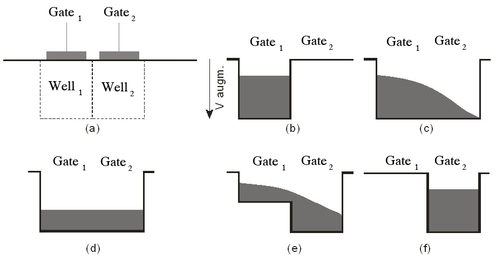
\includegraphics[scale=0.45]{imagens/ccd.jpg}
		\caption{Fluxo de carga de pixels adjacentes.}
	\end{figure}
		
	Como apresentado de forma gráfica em \cite{Spectral}, o funcionamento dos CCDs pode ser descrito, de forma análoga, como uma matriz de baldes (pixels) coletando água da chuva (fótons). Os baldes são expostos à chuva pela mesma quantidade de tempo, e consequentemente se enchem com diferentes quantidades de água. A seguir o CCD inicia a leitura de cada balde por vez. Este processo de leitura é feito transferindo a água de cada balde, da coluna mais a esquerda para o balde adjancente em uma coluna vazia ao lado. Essa coluna anteriormente vazia desloca um de seus baldes para baixo por vez, onde se encontra um conversor que reconhece e armazena o nível d'água. Ou seja, há um deslocamento horizontal dos baldes de uma coluna para baldes de outra, e posteriormente um deslocamento vertical de um balde por vez na coluna de saída.
	
	Na prática, como apresentado na Figura 4, o fótodiodo polarizado reversamente de cada pixel é exposto aos fótons incidentes sobre o sensor. Devido ao fluxo de fótons sobre o fótodiodo, elétrons são liberados - proprocionalmente a intensidade da luz - e, consequentemente, lacunas são criadas na estrutura cristalina. Ou seja, há um fluxo de corrente induzido no fótodiodo agindo como capacitor. Inicialmente, esses elétrons ficam desprendidos na camada de depleção, mas posteriormente são concentrados na parte N+ do fótodiodo por conta do potencial positivo que é induzido nesta parte durante a leitura.
	
	\begin{figure}[H]
	\centering
	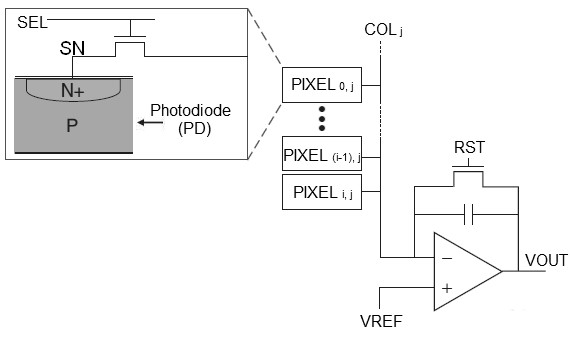
\includegraphics[scale=0.5]{imagens/passive-pixel.jpg}
	\caption{\textit{Array} simplificada de um CCD.}
	\end{figure}
	
	Através do acionamento do transistor de seleção pela entrada SEL as cargas na coluna mais próxima ao amplificador ($COL_{j}$) são deslocadas para um registrador de deslocamento, que será responsável por transferir a carga de um pixel da coluna por vez ao amplificador. Devido ao acionamento do transistor de seleção - que age como o \textit{gate} descrito anteriormente-, após as cargas da coluna serem transferidas para a saída, as cargas nas coluna anteriores ($COL_{j-1}$, $COL_{j-2}$, e assim por diante) são deslocadas para as colunas posteriores ($COL_{j}$, $COL_{j-1}$, e assim por diante). O processo segue em \textit{loop} até que todas as linhas e colunas tenham sido iteradas. A leitura das cargas no CCD pode ser feita de forma mais rápida ao construir o CCD com amplificadores em cada vértice da matriz de pixels, e adicionar registradores de deslocamento em cada aresta.
	
	Após o processo, afim de preparar os pixels do CCD para uma nova leitura, o transistor de \textit{reset} é acionado pela entrada RST, e todos os \textit{gates} são levados à nivel lógico alto - entrada SEL acionada para todas os pixels - por um período de tempo, fazendo com que os fótodiodos de cada pixel voltem para o estado inicial e fiquem prontos para um novo processo.
	
	\subsection*{Sensores CMOS}
	Os sensores CMOS também são constituídos de uma matriz de pixels feita em uma placa de silício. A grande diferença na arquitetura desses dispostivos é que utilizar a configuração APS - ao invés da PPS, como os CCDs -, ou seja, possuem amplificação interna em cada pixel. A seguir, na figura 5, é apresentado um pixel simplificado de um sensor CMOS-3T (3T é devido aos 3 transistores presentes no pixel).
	
	\begin{figure}[!h]
		\centering
		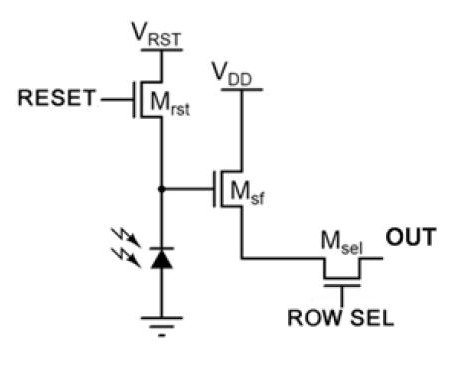
\includegraphics[scale=0.09]{imagens/cmos_3t.jpg}
		\caption{Pixel CMOS 3T.}
	\end{figure}
	
	O princípio de funcionamento dos sensores CMOS é de certa forma mais simples que os CCDs. O fótodiodo polarizado reversamente armazena a tensão $V_{RST}$ ao acionar o transistor MOSFET $M_{rst}$ através da adição de nível HIGH na entrada RESET durante o intervalo de \textit{reset}. Ao levar o nível da entrada RESET para LOW, o fótodiodo é deixado flutuando e os fótons incidentes sobre a junção pn induzem uma corrente que descarrega a tensão armazenada e, consequentemente, altera a tensão no \textit{gate} do transistor $M_{sf}$, que atua como amplificador \textit{source follower}, resultando em uma variação na tensão -submúltiplo de $V_{DD}$ proporcional a tensão no gate do MOSFET- que chega ao transistor de seleção $M_{sel}$. O período de tempo após desligar o transistor $M_{rst}$, onde ocorre a flutuação de tensão no fótodiodo, é chamado tempo de integração.
	
	Após o tempo de integração, acionando o transistor $M_{sel}$ através da entrada ROW SEl, uma corrente flui de VDD para OUT pelos transistores $M_{sel}$ e $M_{sf}$, e a tensão no cátodo do fótodiodo pode ser lida na saída do pixel. A leitura de cada pixel organizados em matrizes é feita linha a linha através do acionamento do $M_{sel}$ correspondente e impondo a corrente em cada coluna. É interssante observar que, diferentemente dos CCDs, os sensores CMOS podem ler várias colunas ao mesmo tempo desde que as colunas não compartilhem a mesma saída de dados para processamento no circuito integrado.
	
	Antes de iniciar um novo ciclo de leitura, um novo tempo de \textit{reset} é distribuído linha a linha, ou em todos os pixels ao mesmo tempo após a leitura de toda a matriz. Ao resetar todos os fótodiodos ao mesmo tempo evitam-se distorções de imagens, processo denominado \textit{global shutter}.
	
	Diferentes configurações de sensores CMOS podem ser obtidas adicionando mais transistores para contemplar novas funções. Por exemplo, os CMOS-4T possuem um transistor de transferência $M_{tx}$ localizado entre o fótodiodo e o \textit{gate} do transistor $M_{sf}$, e um nó FD localizado no encontro do \textit{gate} de $M_{sf}$, \textit{source} de $M_{tx}$ e \textit{drain} de $M_{rst}$. A operação dessa configuração é praticamente a mesma que o CMOS-3T, mas com o transistor de transferência seccionando -$M_{tx}$ desligado- inteiramente o fótodiodo durante a flutuação de tensão na captura de fótons, e interligando-o ao circuito durante a transferência de cargas para o \textit{source follower} e o \textit{reset}. A adição desses novos componentes a estrutura resultam em uma transferência de carga do fótodiodo para a saída OUT com menos ruído.
	
	Outras funções como linhas compartilhadas, 4 e 8 caminhos compartilhados para a leitura mais rápida, aumento da densidade de pixels, ou correção de distorções como \textit{rolling shutter} podem ser adicionadas ao aumentar o número de transistores e/ou empregar outras arquiteturas.
	
	\subsection*{CCD vs. CMOS}
	É possível comparar a eficiência desses dois tipos de sensores ao comparar alguns parâmetros como integração de sistemas, consumo energético, tamanho do circuito integrado, velocidade de processamento, ruído e sensibilidade, e distorção de imagens.
	
	Por conta do uso de PPS (\textit{Passsive Pixels Sesores}), não é possível integrar dispositivos como \textit{timers} e conversores A/D diretamente na matriz de pixels dos sensores CCDs, sendo nessário adicionar \textit{chips} periféricos para realizar essas funções, o que resulta em um tamanho maior para os circuitos integrados CCDs. Já nos sensores CMOS, devido ao processo de fabricação similar ao de circuitos interados, é possível criar o denominado ``\textit{Camera on Chip}'', com todos os periféricos integrados diretamente no \textit{chipset}, resultando em um circuito integrado compacto.
	
	Em relação ao consumo de energia, os CCDs necessitam de diferentes tipos de tensões de alimentação para os diferentes tempos de \textit{clock}, requerindo tensões típicas no \textit{range} de 7 à 10 V, enquanto os sensores CMOS trabalham com tensões mais baixas de 3.3 V à 5 V. Resultando em um consumo de potência menor em sensores CMOS, o que faz prevalecer esses sensores em aplicações que consumo baixo é essencial como circuitos embarcados em celulares.
	
	Comparando a velocidade de processamento, os CCDs utilizam de um processo de deslocamento para o estágio de amplificação e análise como descrito anteriormente. A performance desse deslocamento pode ser melhorada ao adicionar mais registradores de deslocamento no sensor, em troca de aumentar a quantidade de hardware e o tamanho do circuito integrado. Já nos CMOS, a amplificação é feita nos próprios pixels da matriz resultando em uma leitura mais rápida, que pode ser aumentada ainda mais ao utilizar processamento paralelo e analisar múltiplas colunas ao mesmo tempo.
	
	Na teoria, como os sensores CMOS possuem pixels que integram amplificação e ao circuito do fótodiodo, o fator de preenchimento (\textit{Fill Factor}) destes dispositivos acaba sendo menor em comparação aos CCDs, e por conta disso a sensibilidade de sensores CMOS é menor que de CCDs. Além disso os amplificadores utilizados em cada pixel dos sensores CMOS não são idênticos entre si devido às incertezas atreladas ao processo de fabricação de cada MOSFET, por conta disso os fatores de amplificação de cada pixel não são uniformes, resultando em um ruído adicional. Entretanto, na prática, devido à evolução da tecnologia envolvida na fabricação de sensores CMOS, a sensibilidade e ruído de sensores CMOS estão praticamente iguais à dos CCDs.
	
	Para última comparação, faz-se a análise das distorções de imagens causadas por cada sensor. No caso de CCDs, ao expor o sensor por um tempo prolongado haverá um efeito de incandescência (distorções de brilho alto em fotos com fontes luminosas) por conta de sau alta sensibilidade. Já nos sensores CMOS a distorção mais comum é o efeito \textit{rolling shutter} causados pela diferença de tempo entre as leituras de cada linha. Ambos os sensores evoluíram de forma a corrigir as distorções citadas.
	
	De acordo com os argumentos apresentados, conclui-se que sensores CMOS são mais utilizados em aplicações que requerem rápido processamento, baixo consumo elétrico e menor custo de produção como câmeras digitais para celulares, enquanto sensores CCDs são usados em aplicações que necessitam mais sensibilidade, como aplicações de fotografia espacial -entretanto cada vez mais os sensores CMOS evoluem e tomam esse espaço dos CCDs-.
	
	\section*{Conclusão: Simulação de um sensor CMOS 3T simplificado}
	Com o objetivo de consolidar e exemplificar os conhecimentos apresentados de forma teórica ao longo deste trabalho, simula-se um sensor CMOS 3T. A escolha deste sensor foi feita pois sua arquitetura simplificada é facilmente montável e simulável.
		
	Para fazer a simulação foi utilizado o \textit{software} LTSpice a fim de fazer um análise \textit{Transient}. Infelizmente esse \textit{software} não despõem originalmente de fótodiodos e simulações de parâmetros de luminosidade. Para contornar isso, foi utilizada a ferramenta \cite{photodiode} para gerar um circuito equivalente a um fótodiodo polarizado reversamente.
	
	Dentre as configurações dessa ferramenta, escolheu-se a opção de gerar um circuito equivalente ao fótodiodo BPW34S \cite{BPW34} polarizado reversamente por uma tensão de 3.3 V, e com corrente de 45 nA induzida pelo fluxo de fótons durante o período de integração, que consiste em uma fonte de corrente, uma resistência $R_{sh}$ - resistência que aplicada sob a tensão da fonte gera a pequena ``corrente escura'' (\textit{dark current}) característica do fótodiodo em polarização reversa -, e um capacitor $C_{j}$ equivalente a capacitância do fótodiodo em polarização reversa.
	
	\begin{figure}[!h]
		\centering
		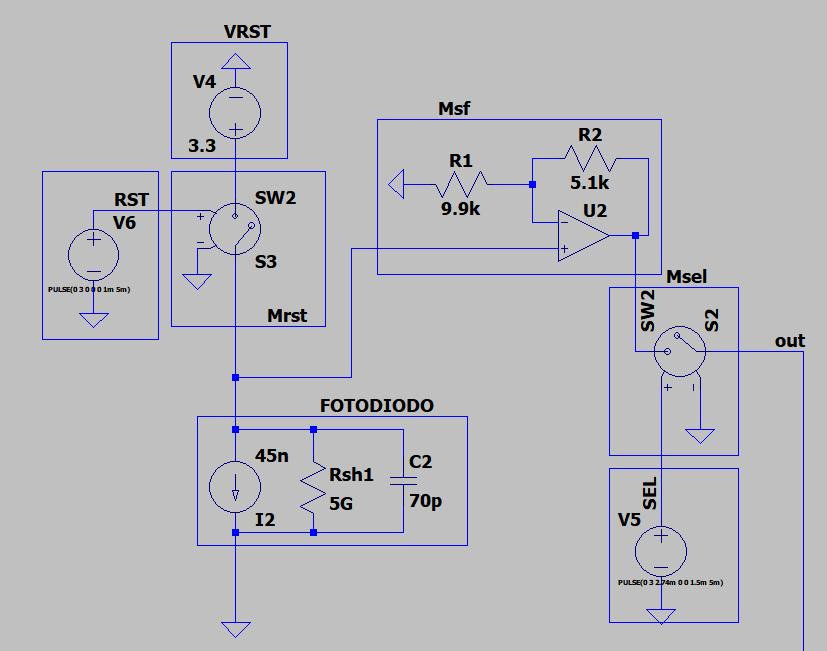
\includegraphics[scale=0.3]{imagens/pixel_simulado.png}
		\caption{Pixel CMOS 3T no LTSpice.}
	\end{figure}
	
	Além disso, os transistores MOSFET $M_{rst}$ e $M_{sel}$ foram substituídos pelo componente ``switch'' (nomeado no LTSpice como sw), e o $M_{sf}$ foi substituído por um amplificador operacional ideal na configuração não inversora que amplifica a tensão para o range de 0 à 5 V. Essas substituições foram feitas a fim de evitar o uso desses transistores não abordados na disciplina de Eletrônica I. A seguir, nas Figura 7 é apresentado o sensor CMOS construído para a simulação.
	
	\begin{figure}[h]
	\centering
	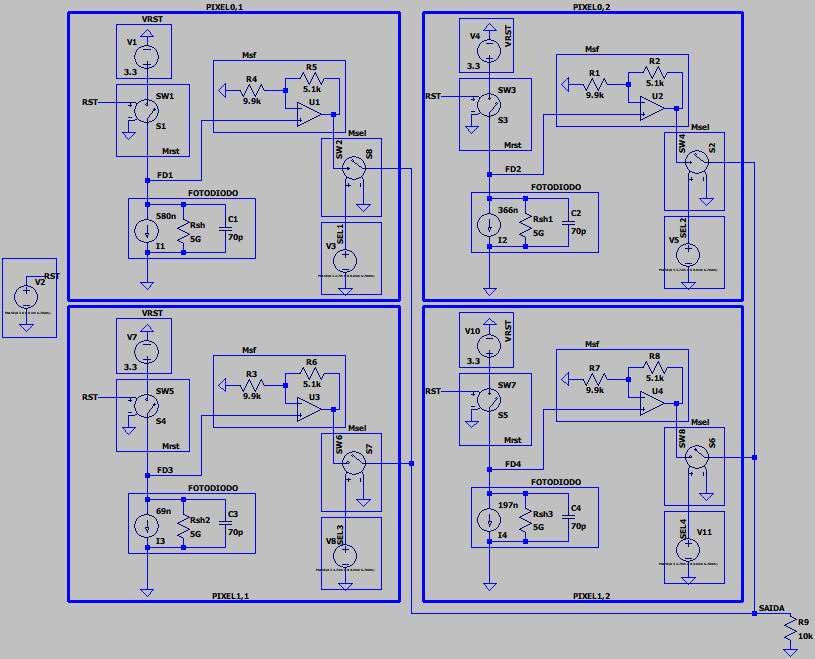
\includegraphics[scale=0.43]{imagens/matriz_simulada.png}
	\caption{Matriz de pixels CMOS 3T no LTSpice.}	
	\end{figure}

	Embora as modificações em relação ao circuito original de um sensor CMOS-3T facilitem mais ainda a montagem do mesmo, elas também adicionam problemas ao circuito como ruído e a necessidadade de trabalhar com tensões reversas, correntes de descarga e tempos de operação com ordem de grandeza diferentes dos empregados na prática. Entretanto, apesar dos problemas criados pelas substituições de componentes, os resultados obtidos são aceitáveis por conta do caráter puramente ilustrativo dessa simulação.

	Para a simulação, o acionamento do ``transistor'' de \textit{reset} é feito seguindo a técnica de \textit{global shutter}, ou seja, todos os pixels são resetados ao mesmo tempo antes da exposição à luminosidade. Após o \textit{reset} de todos os pixel simultaneamente e passar do tempo de integração, inicia-se a leitura de cada pixel linha a linha ao acionar o ``transistor'' de seleção de cada pixel de forma ordenada. O diagrama de \textit{timing} do circuito está ilustrado na Figura 8.
	
	\begin{figure}[H]
	\centering
	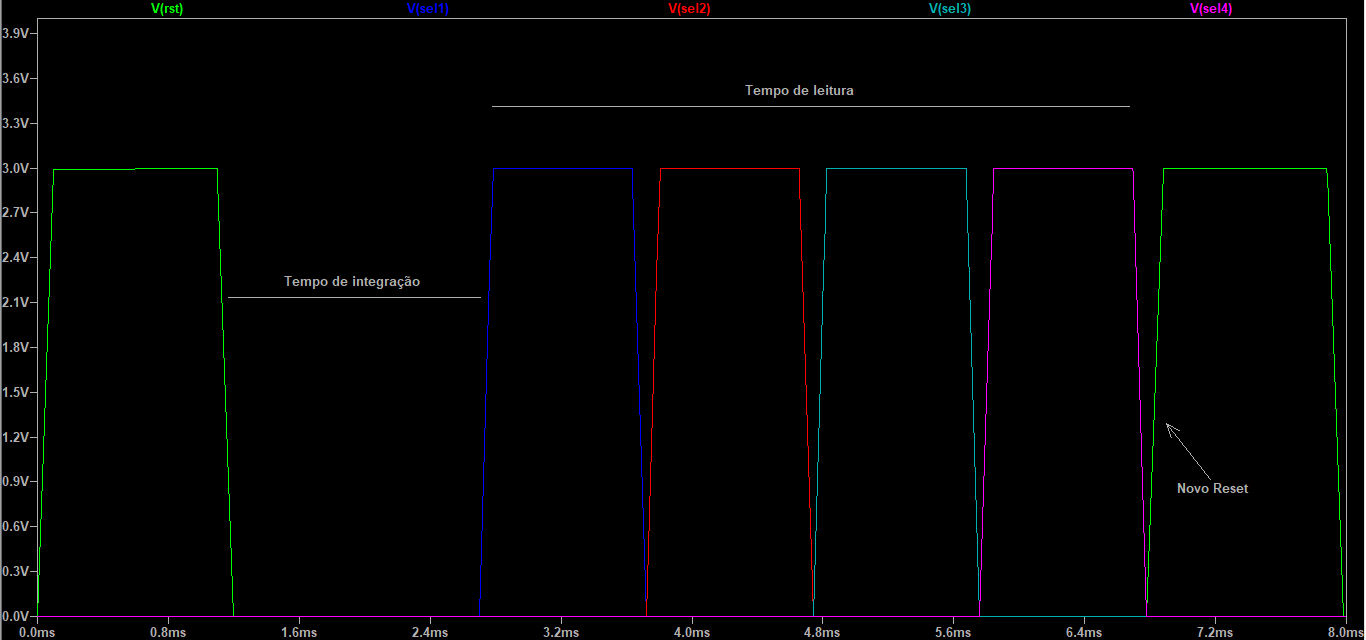
\includegraphics[scale=0.258]{imagens/timings.png}
	\caption{Diagrama de \textit{timings} do acionamento dos ``transistores''.}
	\end{figure}

	Durante o tempo de integração, os fótodiodos são expostos à luz e se descarregam proporcionalmente à corrente induzida pela intensidade luminosa sobre cada pixel (Figura 9). Para simular esse efeito cada pixel da matriz na Figura 7 possui uma corrente de drenagem diferente, produzindo o seguinte gráfico de tensão na saída dos ``fótodiodos''.
	
	\begin{figure}[!h]
		\centering
		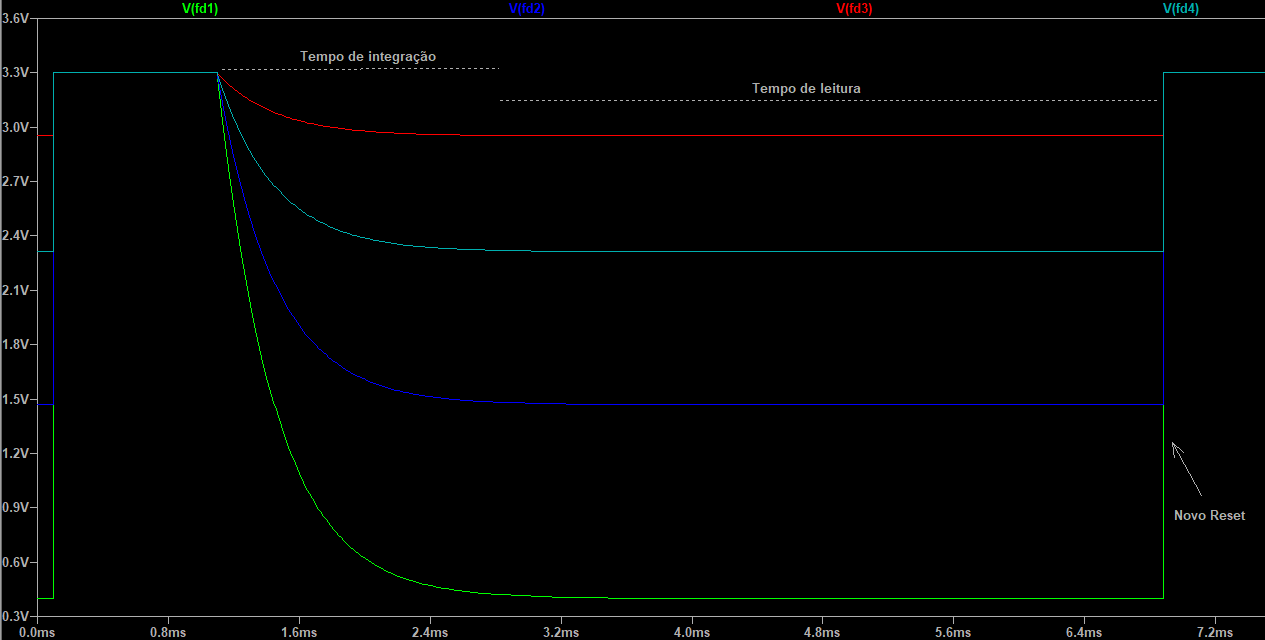
\includegraphics[scale=0.28]{imagens/descarga.png}
		\caption{Descarga da tensão nos fótodiodos causada pela exposição à luz.}
	\end{figure}

	 Após o tempo de integração, as tensões acumulada nos cátodos dos ``fótodiodos'' são direcionadas para o bloco de amplificação de cada pixel, e posteriormente são direcionada para a saída do sensor CMOS durante o intervalo de leitura do respectivo pixel. Na Figura 10 é apresentada a saída da sensor após uma fotografia.
	
	\begin{figure}[!h]
		\centering
		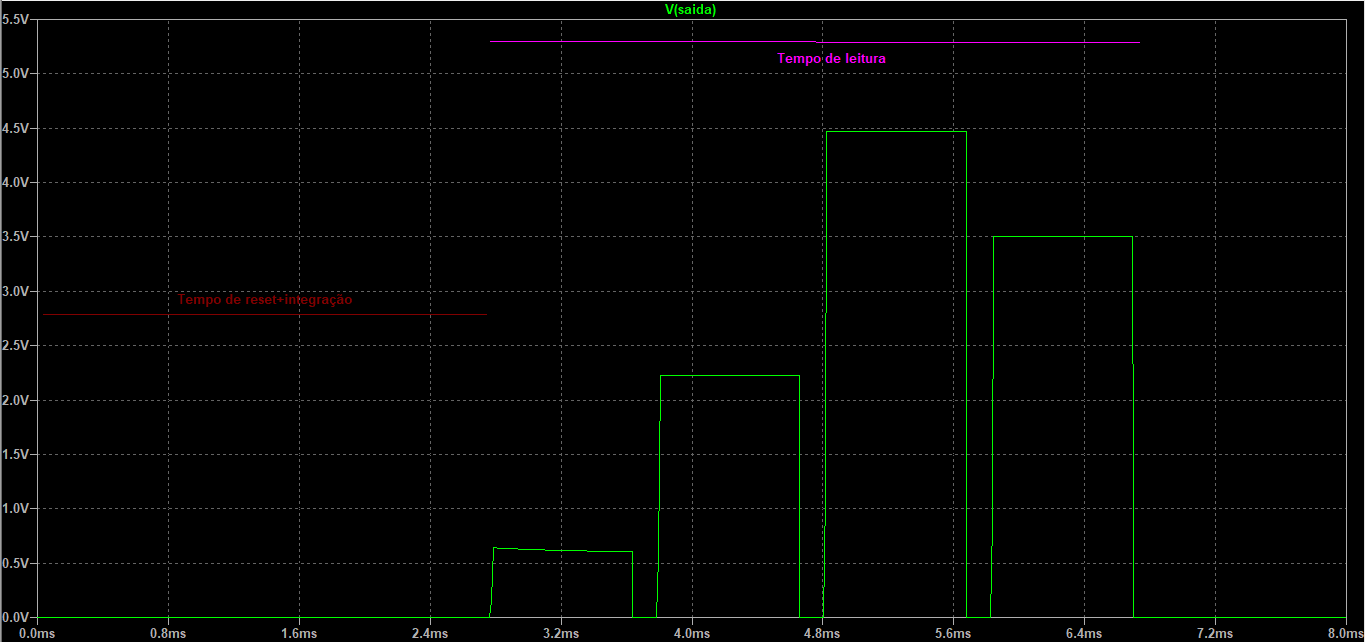
\includegraphics[scale=0.256]{imagens/saida.png}
		\caption{Saída do sensor após uma foto.}
	\end{figure}
		
	\subsection*{Análise dos resultados da simulação}
	 Com a execução da simulação descrita anteriormente obteve-se a tensão armazenada em cada pixel durante o tempo de integração. Analisando essas tensões em um conversor A/D poderia ser feito o armazenamento da cor de cada pixel como uma matriz do filtro de Bayer \cite{bayer} de forma digital para um processamento em software.
	 
	 De forma simplificada, o filtro de Bayer é uma matriz de cores sobreposta à matriz de pixels do sensor de imagem de forma a cada elemento da matriz do filtro de Bayer ``filtrar'' a cor da luz que chega ao seu respectivo pixel. Os elementos da matriz do filtro são as cores usadas no padrão RGB, vermelho, verde e azul. Assim, quando é analisada a intensidade da luz que chegou em um pixel do sensor, na verdade é medida a quantidade exata do componente da cor do filtro existente na luz. Ao fazer isso em uma matriz disposta de forma padronizada com as cores RGB é possível quantificar as cores em cada região da imagem e posteriormente, através do algoritmo de \textit{demosaicing} \cite{bayer} em software, converter a imagem para o formato RGB (uma imagem digital com resolução em pixels igual à do sensor, mas com cada pixel tendo valores de intensidade de verde, vermelho e azul simultaneamente).
	 
	 Para exemplificar com os resultados obtidos da simulação (Figura 10), considera-se um filtro de Bayer disposto sobre a matriz de pixels simulada como tendo os pixels da diagonal principal da matriz ($PIXEL_{0,0}$ e $PIXEL_{1,1}$) na cor verde, o pixel restante da segunda linha ($PIXEL_{1,0}$) como vermelho, e o restante da primeira linha ($PIXEL_{0,1}$) como azul. Então ao analisar as tensões de saída do sensor, observa-se que as tensões dos pixels da segunda linha (2 últimos valores) estão  próximas de 5 V, isso significa que aquela região da foto recebeu menos intensidade luminosa, e que as dos pixels da primeira linha (2 primeiros valores) estão no intervalo de 0 V à 2.5 V, ou seja, uma região da foto com mais intensidade luminosa. Ao converter esses valores de tensão para o formado RGB (variando de 0 à 255), obtém-se as cores apresentadas na matriz digitalizada do filtro de Bayer na Figura 11.
	 
 	\begin{figure}[!h]
 	\centering
 	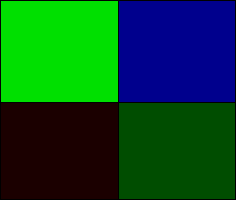
\includegraphics[scale=0.4]{imagens/filtro_bayer.png}
 	\caption{Matriz digitalizada com as cores de cada pixel.}
	 \end{figure}
	 
	\begin{thebibliography}{99}
		\bibitem[1]{MazinSaad2019}
		{Mazin H.; Saad D. {Design and simulation of a CMOS image sensor with a built-in edge detection for tactile vision sensory substituition}, \textbf{AIMS Electronics and Electrical Engineering}. DOI: 10.3924/ElectrEng.2019.2.144, 06 May 2019.}
		\bibitem[2]{Spectral}
		{Spectral Instruments, Inc. {What is a CCD?}, Disponível em: \url{https://specinstcameras.com/what-is-a-ccd/}, 2021. Acesso em: 07 mar 2022.}
		\bibitem[3]{ImageSensorWiki}
		{IMAGE sensor. In:WIKIPÉDIA: a enciclopédia livre. Wikimedia, 2006. Disponível em: \url{https://en.wikipedia.org/wiki/Image_sensor} Acesso em: 07 mar 2022.}
		\bibitem[4]{ActivePixelWiki}
		{ACTIVE-pixel sensor. In:WIKIPÉDIA: a enciclopédia livre. Wikimedia, 2006. Disponível em: \url{https://en.wikipedia.org/wiki/Active-pixel_sensor} Acesso em: 04 mar 2022.}
		\bibitem[5]{StefanoMeroli}
		{Meroli, Stefano, {Design and implementation of Active Pixel Sensors (APS)}, Disponível em: \url{https://meroli.web.cern.ch/lecture_activepixelsensors.html}. Acesso em: 07 mar 2022.}
		\bibitem[6]{ColorRecognition}
		{Computerphile, {Capturing Digital Images (The Bayer Filter) - Computerphile}. Youtube, 2015. Disponível em: \url{https://www.youtube.com/watch?v=LWxu4rkZBLw}. Acesso em: 07 mar 2022.}
		\bibitem[7]{CCDvsCMOS}
		{ALL ABOUT ELECTRONICS, {Image Sensors Explained: How CCD and CMOS Sensors works? CCD vs CMOS}. Youtube, 2019. Disponível em: \url{https://www.youtube.com/watch?v=FKJFIzDfUNE&t=421s}. Acesso em: 05 mar 2022.}
		\bibitem[8]{BPW34}
		{Vishay Semiconductors, {``BPW34, BPW34S: Silicon PIN Photodiode''}, Data Sheet, Document Number: 91000, 01 Jan 2022. Disponível em: \url{https://www.vishay.com/docs/81521/bpw34.pdf}. Acesso em: 10 mar 2022.}
		\bibitem[9]{photodiode}
		{Analog Devices. {Photodiode Circuit Design Wizard}, Website. Disponível em: \url{https://tools.analog.com/en/photodiode/}. Acesso em: 10 mar 2022}
		\bibitem[10]{bayer}
		{BAYER filter. In:WIKIPÉDIA: a enciclopédia livre. Wikimedia, 2006. Disponível em: \url{https://en.wikipedia.org/wiki/Bayer_filter} Acesso em: 11 mar 2022.}

	\end{thebibliography}
\end{document}